% Author: Marek Fiser <tikz at marekfiser.cz>
% MESIF protocol: http://en.wikipedia.org/wiki/MESIF_protocol
\documentclass[tikz, border=100pt]{standalone}
%%%<
\usepackage{verbatim}
%%%>
\begin{comment}
:Title: MESIF protocol
:Tags: Diagrams;Block diagrams;Computer science
:Author: Marek Fiser
:Slug: mesif

A diagram describing the MESIF protocol: http://en.wikipedia.org/wiki/MESIF_protocol
\end{comment}
\usetikzlibrary{arrows}
\begin{document}
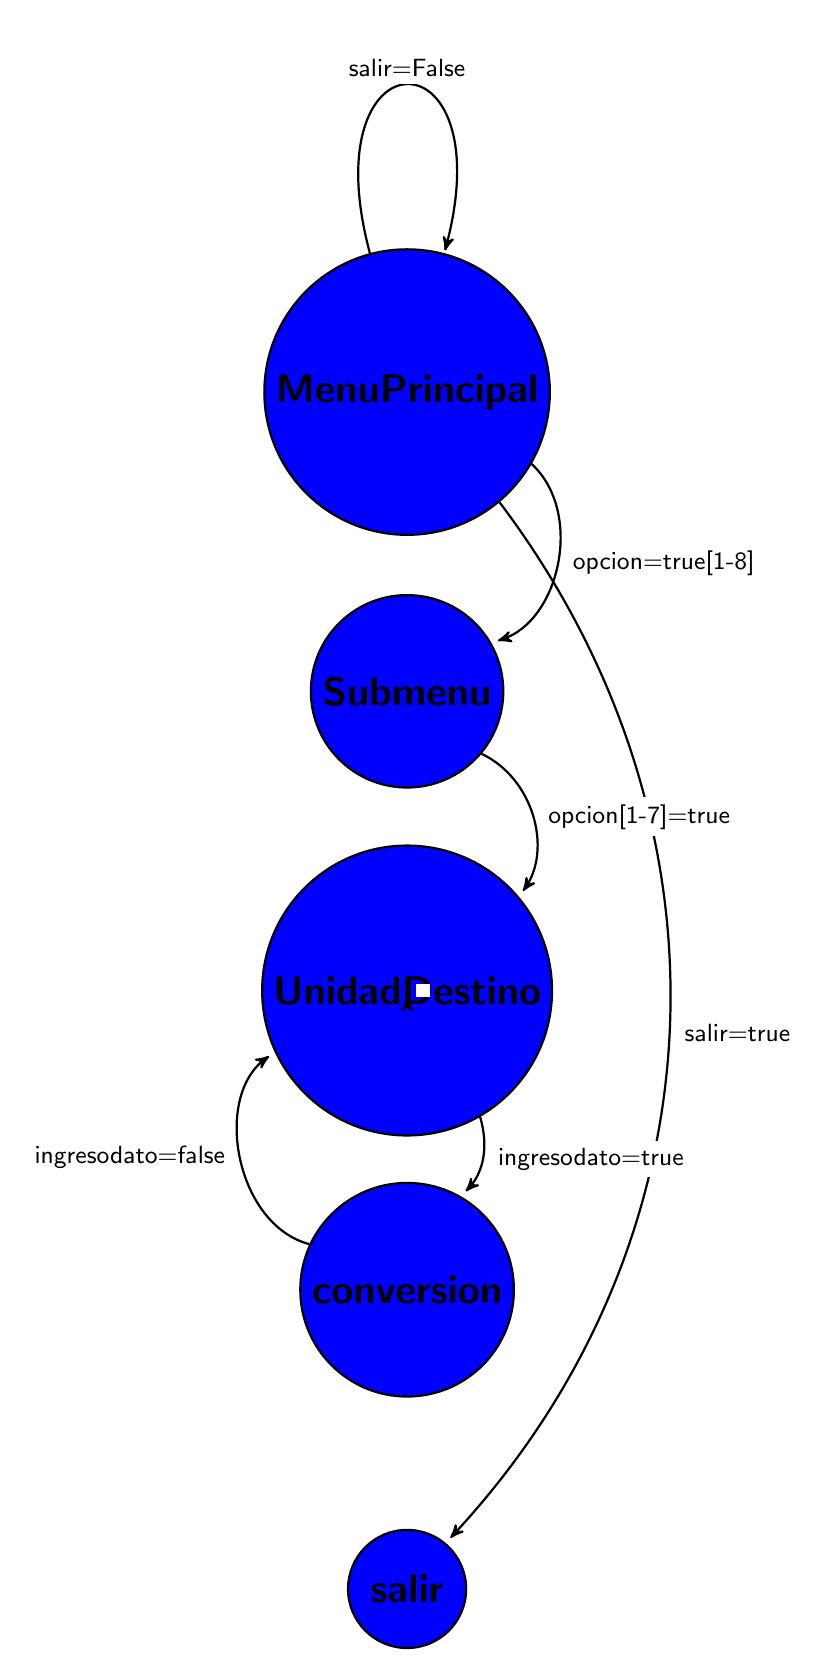
\begin{tikzpicture}[->,>=stealth',shorten >=2.5pt,auto,node distance=3.8cm,
  thick,main node/.style={circle,fill=blue!155,draw,
  font=\sffamily\Large\bfseries,minimum size=15mm}]

  \node[main node] (MenuPrincipal) {MenuPrincipal};
  \node[main node] (Submenu) [below of=MenuPrincipal] {Submenu};
  \node[main node] (UnidadDestino) [below of=Submenu] {UnidadDestino};
  \node[main node] (conversion) [below of=UnidadDestino] {conversion};
  \node[main node] (salir) [below of=conversion] {salir};

  \path[every node/.style={font=\sffamily\small,
  		fill=white,inner sep=2.5pt}]
  	% Right-hand-side arrows rendered from top to bottom to
  	% achieve proper rendering of labels over arrows.
    (MenuPrincipal) edge [loop above] node {salir=False} (MenuPrincipal)
        edge [bend left=60] node[right=1mm] {opcion=true[1-8]} (Submenu)
        edge [bend left=40] node[right=1mm] {salir=true} (salir)
        
    (Submenu) 
        edge [bend left=50] node[right=1mm] {opcion[1-7]=true} (UnidadDestino)
        %edge [bend left=30] node[right=1mm] {ingresodato=true} (conversion);
        
    (UnidadDestino) 
        edge [bend left=45] node[right=1mm] {} (UnidadDestino)
        edge [bend left=30] node[right=1mm] {ingresodato=true} (conversion)   
         
        
    %(S) edge [loop above] node {PrRd/-} (S)
     %   edge [loop right] node[right=1mm]  {BusRd/-} (S)
      %  edge [bend left=40] node[right=1mm] {BusRdX/Flush} (I)
    %(F) edge [bend left=30] node[right=1mm] {BusRdX/Flush} (I)
        
  	% Left-hand-side arrows rendered from bottom to top to
  	% achieve proper rendering of labels over arrows.
  	(conversion)edge [bend left=65] node[left=1mm] {ingresodato=false} (UnidadDestino);    
    %(I) edge [bend left=65] node[left=1mm] {PrWr/BusRdX} (M)
    %    edge [bend left=55] node[left=1mm] {PrRd/BusRd Ex} (E)
     %   edge [bend left=30] node[left=1mm] {PrRd/BusRd} (F)
    %(F) edge [loop above] node {PrRd/-} (F)
     %   edge [bend left=50] node[left=1mm] {PrWr/BusRdX} (M)
      %  edge [bend left=30] node[left=1mm] {BusRd/Flush} (S)
    %(S) edge [bend left=40] node[left=1mm] {PrWr/BusRdX} (M)
   % (E) edge [bend left=30] node[left=1mm] {PrWr/-} (M);
\end{tikzpicture}
\end{document}